\documentclass[border=0.8ex,svgnames,tikz]{standalone}
\usepackage{amsmath,mathtools}
\usepackage{fontspec}
\setmainfont{Source Serif 4}
\setsansfont{Source Sans 3}
\setmonofont{Source Code Pro}
\usetikzlibrary{calc,matrix,positioning}
\begin{document}
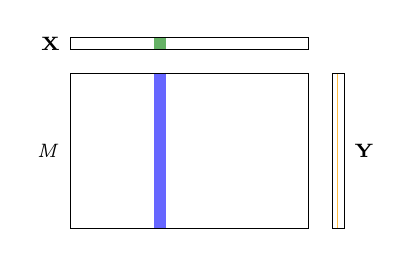
\begin{tikzpicture}
  \begin{scope}[
    every matrix/.style={
      matrix of math nodes,
      nodes in empty cells,
      inner sep=0,
      outer sep=0,
      column sep=0,
      row sep=0,
      nodes={
        minimum width=1ex,
        minimum height=1ex,
        anchor=center,
        inner sep=0pt,
        outer sep=0pt,
        font=\small,
      },
    },
    ]
    \begin{scope}[column 8/.style={nodes={fill=Green!60}}]
      \matrix (X) {
        & & & & & & & & & & & & & & & & & & & \\
      };
      \node[left=0.05ex of X.west] {\scriptsize \textbf{X}};
      \draw (X.south west) |- (X.north east);
      \draw (X.south west) -| (X.north east);
    \end{scope}
    \begin{scope}[column 8/.style={nodes={fill=Blue!60}}]
      \matrix [below=2ex of X] (M) {
        & & & & & & & & & & & & & & & & & & & \\
        & & & & & & & & & & & & & & & & & & & \\
        & & & & & & & & & & & & & & & & & & & \\
        & & & & & & & & & & & & & & & & & & & \\
        & & & & & & & & & & & & & & & & & & & \\
        & & & & & & & & & & & & & & & & & & & \\
        & & & & & & & & & & & & & & & & & & & \\
        & & & & & & & & & & & & & & & & & & & \\
        & & & & & & & & & & & & & & & & & & & \\
        & & & & & & & & & & & & & & & & & & & \\
        & & & & & & & & & & & & & & & & & & & \\
        & & & & & & & & & & & & & & & & & & & \\
        & & & & & & & & & & & & & & & & & & & \\
      };
      \node[left=0.05ex of M.west] {\scriptsize \textit{M}};
      \draw (M.south west) |- (M.north east);
      \draw (M.south west) -| (M.north east);
    \end{scope}
    \begin{scope}
      \matrix [right=2ex of M] (Y) {
        \\
        \\
        \\
        \\
        \\
        \\
        \\
        \\
        \\
        \\
        \\
        \\
        \\
      };
      \foreach \x in {1,...,13} {
        \fill [Orange!75] ($(Y-\x-1.south west)!0.35!(Y-\x-1.south east)$)
        rectangle ($(Y-\x-1.north west)!0.40!(Y-\x-1.north east)$);
      }
    \node[right=0.05ex of Y.east] {\scriptsize \textbf{Y}};
    \draw (Y.south west) |- (Y.north east);
    \draw (Y.south west) -| (Y.north east);
    \end{scope}
  \end{scope}
\end{tikzpicture}
\end{document}
